\section{Additional experiments with tuning}\label{additionalExperiments}

The reference results presented in the previous section represent the performance a user can expect without extensive tuning and configuration efforts. However, enabling or disabling a key feature of a system that the user is familiar with can have a significant impact on performance, just as employing certain alternative configurations can. The purpose of the additional experiments we present in this section is to examine some of such options that the user may make use of.

\subsection{Databricks with table and column statistics}\label{databricksWithStatistics}

Modern SQL-compliant big data processing frameworks incorporate many of the developments in query processing techniques for database management systems that have arisen through now decades of research. Query optimization is particularly important since it facilitates data independence, allowing declarative queries to run usually as fast as a custom program to evaluate a query. However, the optimizer requires an appropriate characterization of the database properties and distribution in the form of table and column statistics.

Table statistics refer to basic information such as the number of rows in a table, the number of files comprising the table, and their size. These are not produced by Databricks by default but can be created with an ANALYZE TABLE \textless table name\textgreater \ COMPUTE STATISTICS statement. Column statistics, on the other hand, cover a particular attribute of a table, involving minimum and maximum values, number of null values, and sketches and histograms of distributions. In Databricks, their creation requires an ANALYZE TABLE \textless table name\textgreater \ COMPUTE STATISTICS FOR COLUMNS \textless columns\textgreater \ statement, thus the specific columns need to be specified.

In the experiments we present next, we generated table and column statistics for all tables and all columns, and enabled the cost-based query optimizer. First, we show the time required to generate these table and column statistics in Figure \ref{fig:additionalResultsDatabricksWithStatsDataLoading}.

\begin{figure}
   \begin{center}
   \scalebox{0.65}{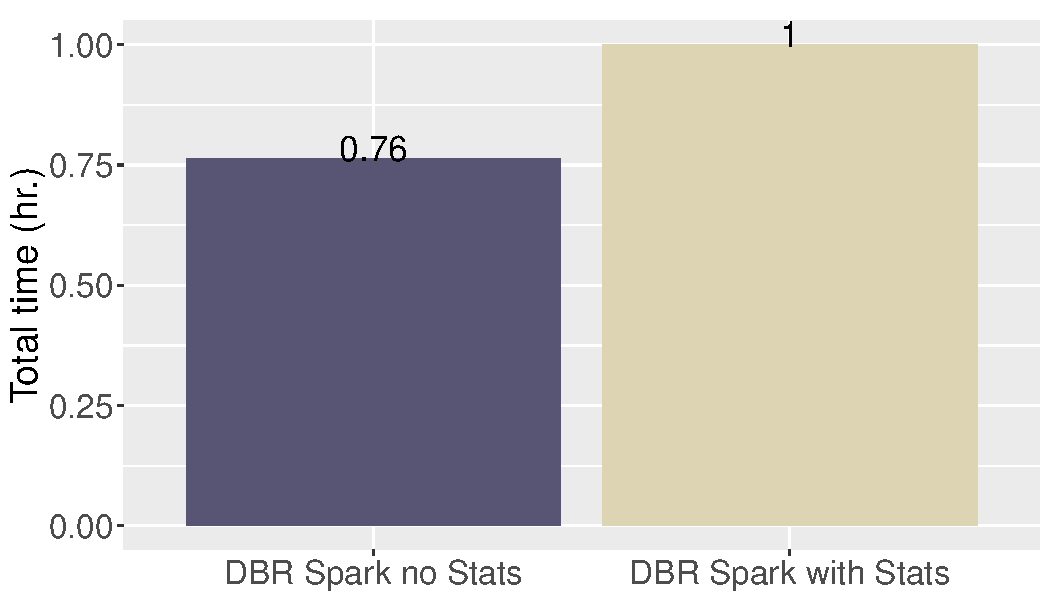
\includegraphics[width=7.0in]{imgs/additionalExperiments/statsResultsGraphs/load_totalHrTimeBarChart.pdf}}
   \end{center}
   \caption{Databricks Data Loading Test with and without statistics generation.}
   \label{fig:additionalResultsDatabricksWithStatsDataLoading}
\end{figure}

We can see that the generation of statistics takes about 15 minutes, increasing the total data loading time to one hour. In our current implementation, all of the tables are created first and then an additional application analyzes them. The statistics creation time could be reduced by restricting the analyzed columns and tables, but in any case, it is relatively low considering the size of the data. The effect of cost-based query optimization relying on these statistics on the Power Test is summarized in Figure \ref{fig:additionalResultsDatabricksWithStatsPowerTestTotalTime} to Figure \ref{fig:additionalResultsDatabricksWithStatsPowerTestArithmeticMean}.

\begin{figure}
   \begin{center}
   \scalebox{0.65}{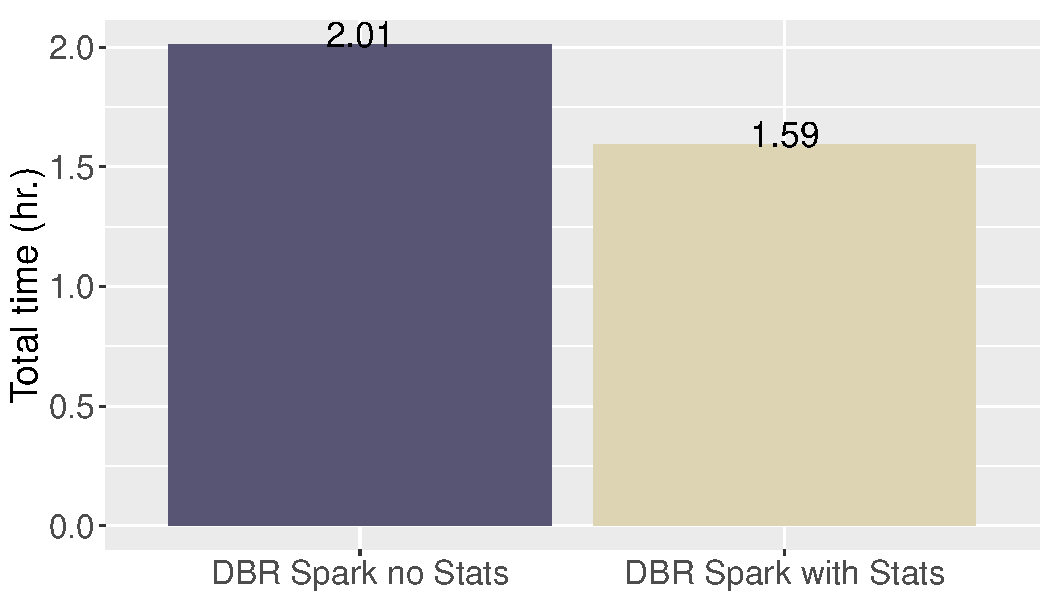
\includegraphics[width=7.0in]{imgs/additionalExperiments/statsResultsGraphs/power_totalHrTimeBarChart.pdf}}
   \end{center}
   \caption{Databricks Power Test total time with and without statistics.}
   \label{fig:additionalResultsDatabricksWithStatsPowerTestTotalTime}
\end{figure}

\begin{figure}
   \begin{center}
   \scalebox{0.65}{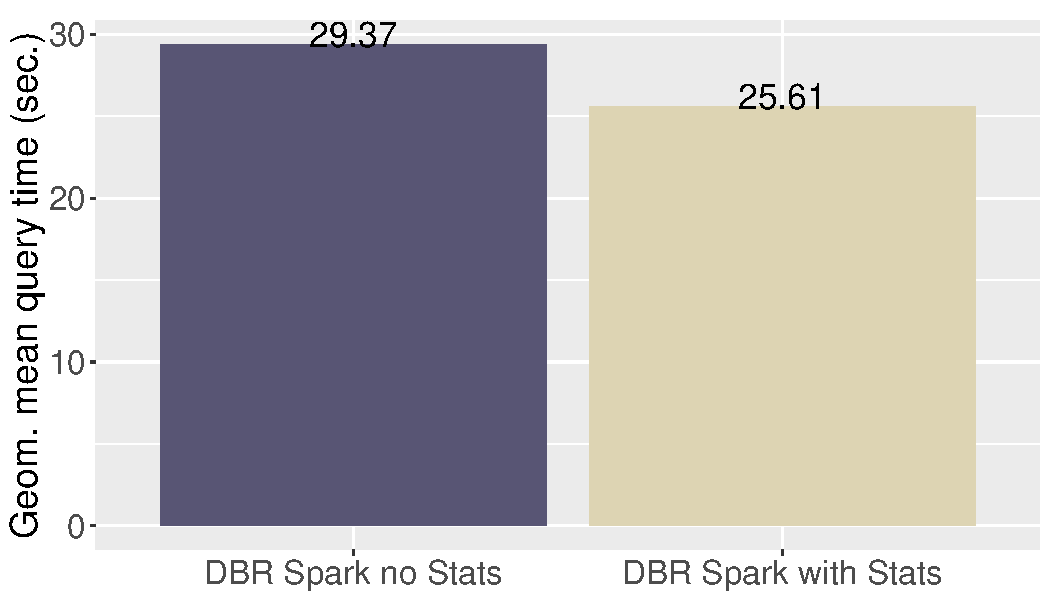
\includegraphics[width=7.0in]{imgs/additionalExperiments/statsResultsGraphs/power_geomeanTimeBarChart.pdf}}
   \end{center}
   \caption{Databricks Power Test query execution time geometric mean with and without statistics.}
   \label{fig:additionalResultsDatabricksWithStatsPowerTestGeomean}
\end{figure}

\begin{figure}
   \begin{center}
   \scalebox{0.65}{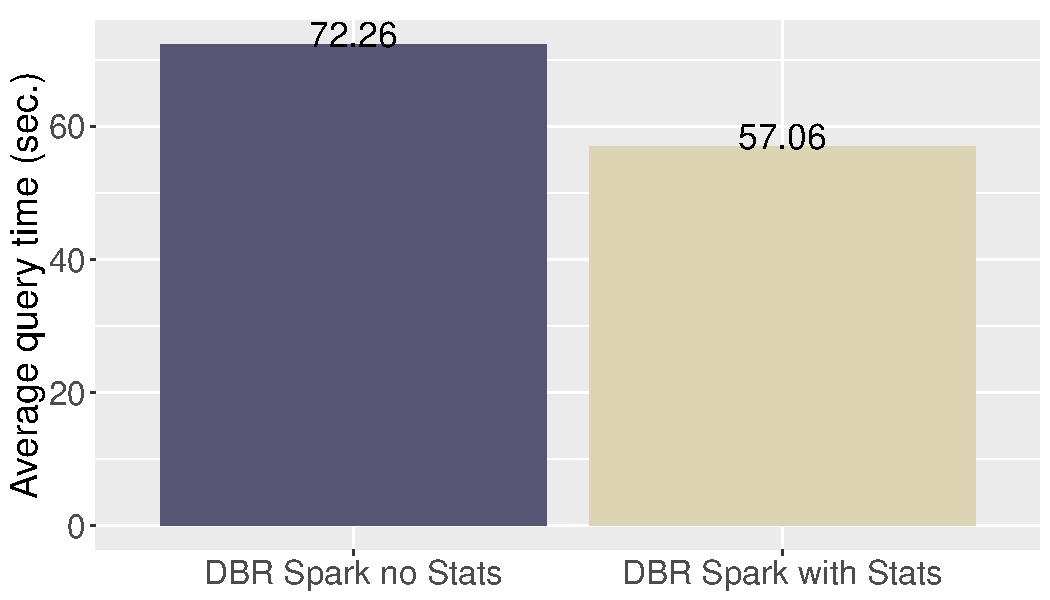
\includegraphics[width=7.0in]{imgs/additionalExperiments/statsResultsGraphs/power_avgTimeBarChart.pdf}}
   \end{center}
   \caption{Databricks Power Test query execution time arithmetic mean with and without statistics.}
   \label{fig:additionalResultsDatabricksWithStatsPowerTestArithmeticMean}
\end{figure}

The total execution time for the Power Test is reduced from two hours to around one hour and 36 minutes, or approximately 20\%. The geometric mean of the query execution time and the arithmetic mean are reduced proportionally. Figure \ref{fig:additionalResultsDatabricksWithStatsPowerTestIndividualQueries1} to Figure \ref{fig:additionalResultsDatabricksWithStatsPowerTestIndividualQueries5} depict the effect on the individual queries.

\begin{figure}
   \begin{center}
   \scalebox{0.65}{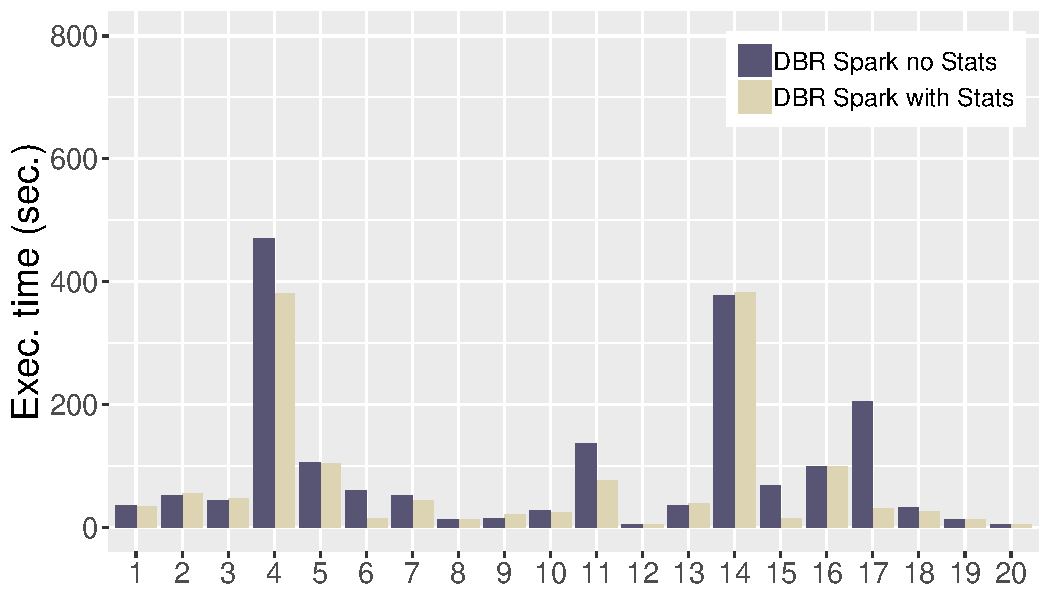
\includegraphics[width=7.0in]{imgs/additionalExperiments/statsResultsGraphs/1_PDFsam_PowerTestCompAll.pdf}}
   \end{center}
   \caption{Databricks Power Test individual query execution times with and without statistics (1).}
   \label{fig:additionalResultsDatabricksWithStatsPowerTestIndividualQueries1}
\end{figure}

\begin{figure}
   \begin{center}
   \scalebox{0.65}{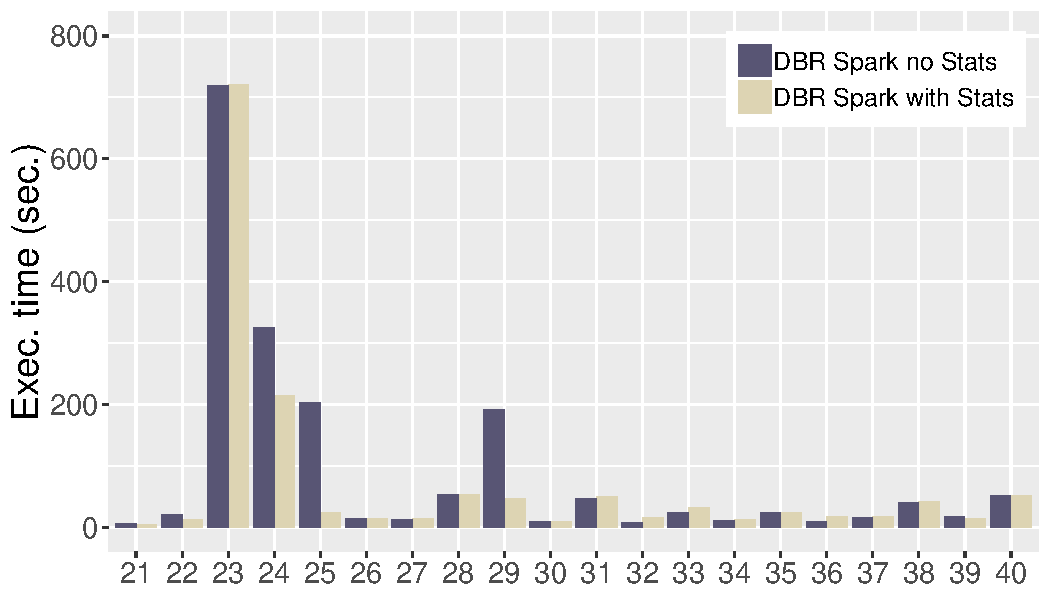
\includegraphics[width=7.0in]{imgs/additionalExperiments/statsResultsGraphs/2_PDFsam_PowerTestCompAll.pdf}}
   \end{center}
   \caption{Databricks Power Test individual query execution times with and without statistics (2).}
   \label{fig:additionalResultsDatabricksWithStatsPowerTestIndividualQueries2}
\end{figure}

\begin{figure}
   \begin{center}
   \scalebox{0.65}{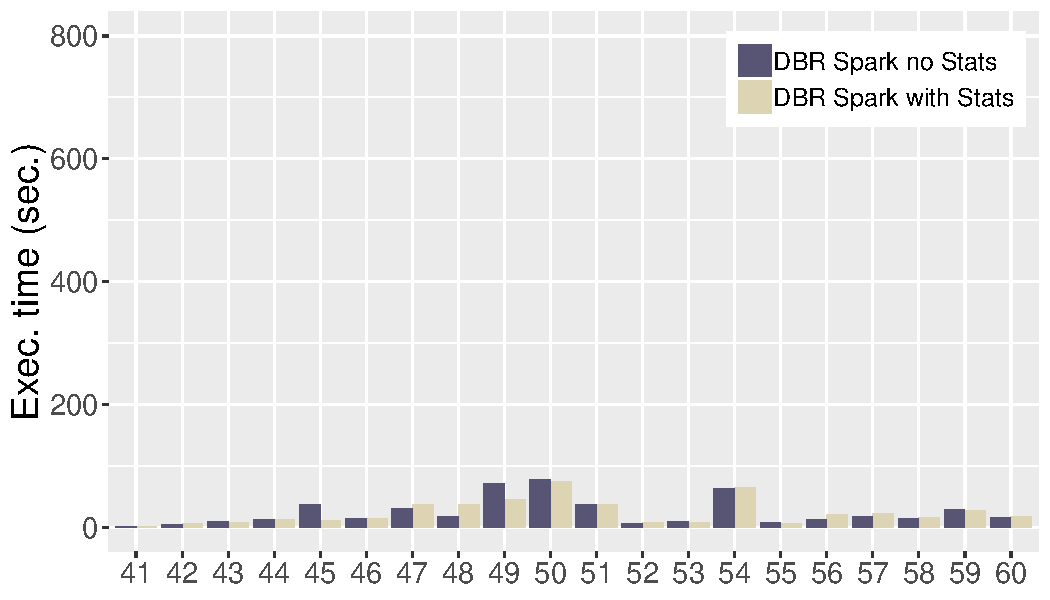
\includegraphics[width=7.0in]{imgs/additionalExperiments/statsResultsGraphs/3_PDFsam_PowerTestCompAll.pdf}}
   \end{center}
   \caption{Databricks Power Test individual query execution times with and without statistics (3).}
   \label{fig:additionalResultsDatabricksWithStatsPowerTestIndividualQueries3}
\end{figure}

\begin{figure}
   \begin{center}
   \scalebox{0.65}{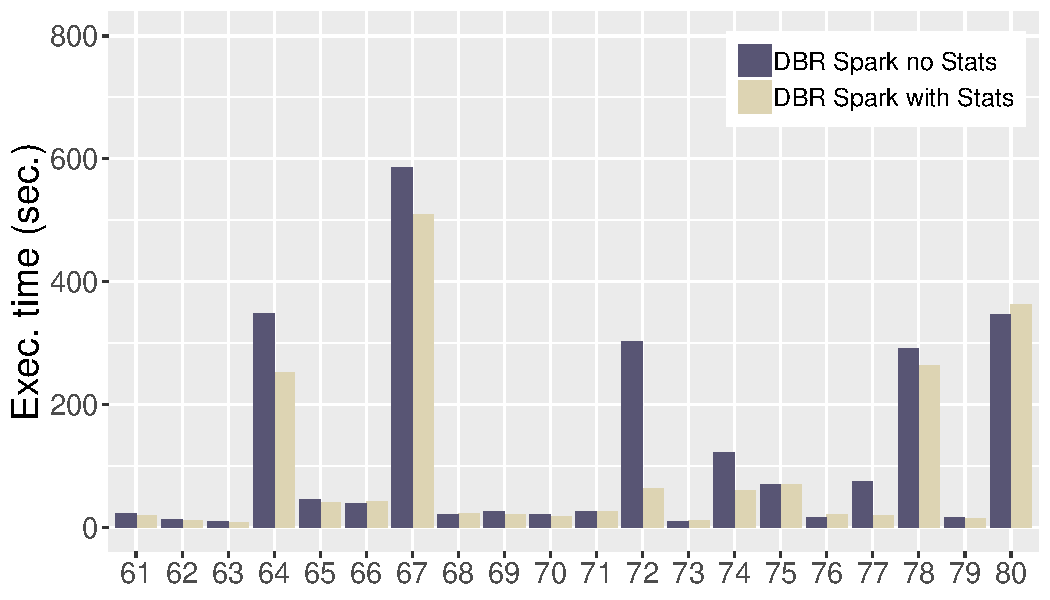
\includegraphics[width=7.0in]{imgs/additionalExperiments/statsResultsGraphs/4_PDFsam_PowerTestCompAll.pdf}}
   \end{center}
   \caption{Databricks Power Test individual query execution times with and without statistics (4).}
   \label{fig:additionalResultsDatabricksWithStatsPowerTestIndividualQueries4}
\end{figure}

\begin{figure}
   \begin{center}
   \scalebox{0.65}{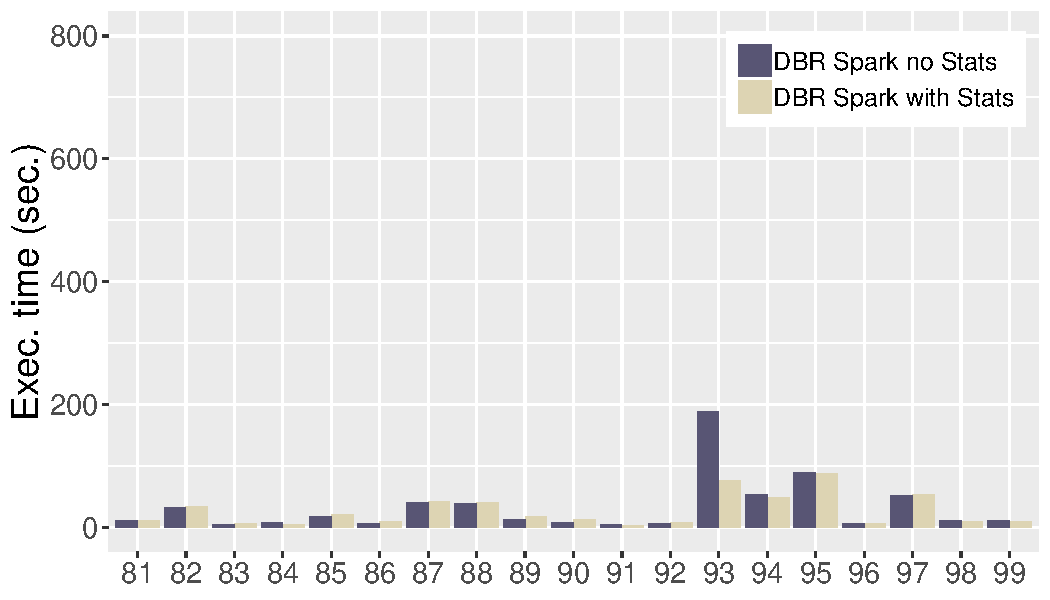
\includegraphics[width=7.0in]{imgs/additionalExperiments/statsResultsGraphs/5_PDFsam_PowerTestCompAll.pdf}}
   \end{center}
   \caption{Databricks Power Test individual query execution times with and without statistics (5).}
   \label{fig:additionalResultsDatabricksWithStatsPowerTestIndividualQueries5}
\end{figure}

In many cases, the execution time is essentially the same, while in others the differences are very significant. Analyzing at a greater depth we find that 48 queries showed slower completion times with statistics and optimization. Although this may seem to support the idea that statistics and optimization can be counterproductive half of the time, the number of queries with a noticeable and accurately measurable slowdown, say at least 10\%, drops to 21. Two queries ran twice as slow, these being 36 and 48.

Conversely, among the 51 queries that saw improvement with the use of statistics and optimization, 33 of them completed in 90\% of the time or less than without them. Furthermore, 11 of them completed in half of the time or less. In particular, query 72 ran almost five times as fast, which is noteworthy given that the query had already been partially optimized manually in order to make it terminate in EMR Presto in a reasonable time. Overall, we can say with confidence that generating table and column statistics is worth it, since although the optimization process is not perfect, it is highly likely that it will yield significant performance improvements. The Throughput Test results, presented in Figure \ref{fig:additionalResultsDatabricksWithStatsTputTest} exemplify this.

\begin{figure}
   \begin{center}
   \scalebox{0.65}{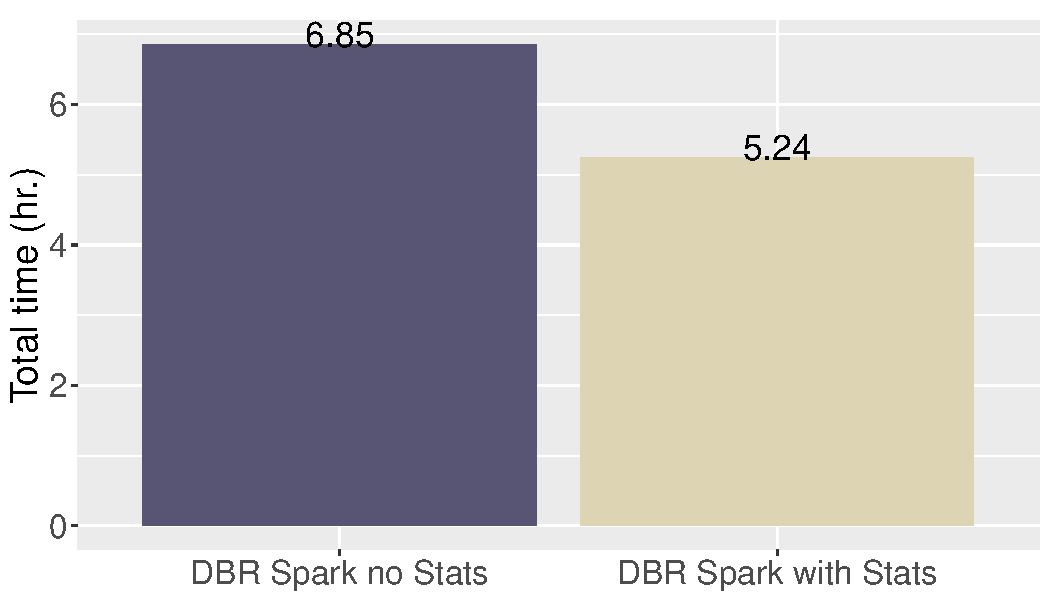
\includegraphics[width=7.0in]{imgs/additionalExperiments/statsResultsGraphs/tput_totalHrTimeBarChart.pdf}}
   \end{center}
   \caption{Databricks Throughput Test total time with and without statistics.}
   \label{fig:additionalResultsDatabricksWithStatsTputTest}
\end{figure}

\subsection{Databricks with table statistics only}

Recalling the results in Figure \ref{fig:additionalResultsDatabricksWithStatsDataLoading} showing the total data loading time with and without table and column statistics generation, the question may arise of what optimization results can be achieved with only table statistics, and how much time will be saved that way in the data loading process. We carried out the experiments in question arriving at two main conclusions. First, although generating table and column statistics is not a very time consuming process, the time becomes negligible when only table statistics are produced. Concretely, it takes about 2 minutes, thus mostly launching and scheduling tasks and no significant amount of data processing.

Second, it can be very counterproductive to employ the cost-based optimizer when only table statistics are available. Figure \ref{fig:additionalResultsDatabricksWithBasicStatsPowerTestTotalTime} shows the results of the Power Test employing only table statistics.

\begin{figure}
   \begin{center}
   \scalebox{0.65}{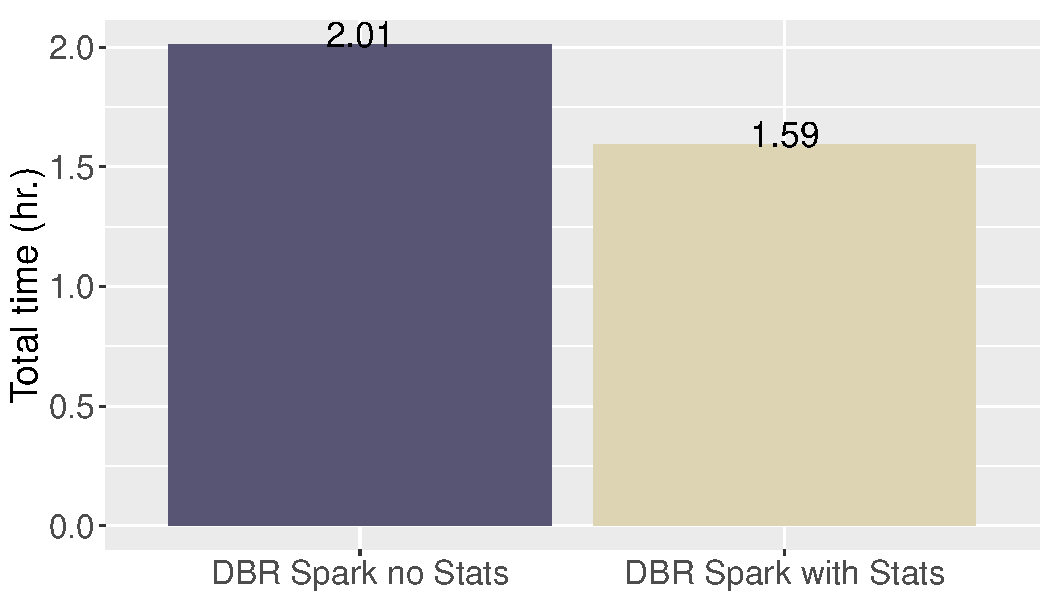
\includegraphics[width=7.0in]{imgs/additionalExperiments/statsResultsGraphs/power_totalHrTimeBarChart.pdf}}
   \end{center}
   \caption{Databricks Power Test total time with and without basic statistics.}
   \label{fig:additionalResultsDatabricksWithBasicStatsPowerTestTotalTime}
\end{figure}

Using the cost-based optimizer with only table statistics at its disposal results in a total execution time more than 3 times greater. However, this large difference is for the most part due to the fact that query 72 takes about 4.6 hours to complete when the optimizer has only table statistics to derive a plan. The difference between the arithmetic and geometric means, shown in Figure \ref{fig:additionalResultsDatabricksWithBasicStatsPowerTestArithmeticMean} and Figure \ref{fig:additionalResultsDatabricksWithBasicStatsPowerTestGeomean}, respectively, captures this anomaly. Figure \ref{fig:additionalResultsDatabricksWithBasicStatsPowerTestIndividualQueries1} to Figure \ref{fig:additionalResultsDatabricksWithBasicStatsPowerTestIndividualQueries5} present a comparison for the individual queries (we exclude query 72 for clarity).

\begin{figure}
   \begin{center}
   \scalebox{0.65}{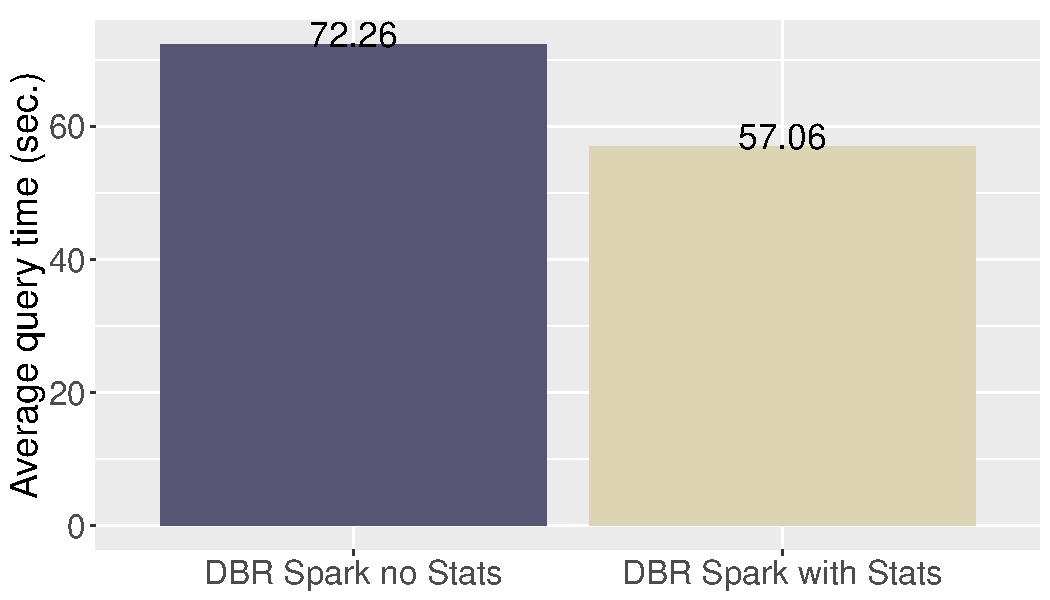
\includegraphics[width=7.0in]{imgs/additionalExperiments/statsResultsGraphs/power_avgTimeBarChart.pdf}}
   \end{center}
   \caption{Databricks Power Test query execution time arithmetic mean with and without basic statistics.}
   \label{fig:additionalResultsDatabricksWithBasicStatsPowerTestArithmeticMean}
\end{figure}

\begin{figure}
   \begin{center}
   \scalebox{0.65}{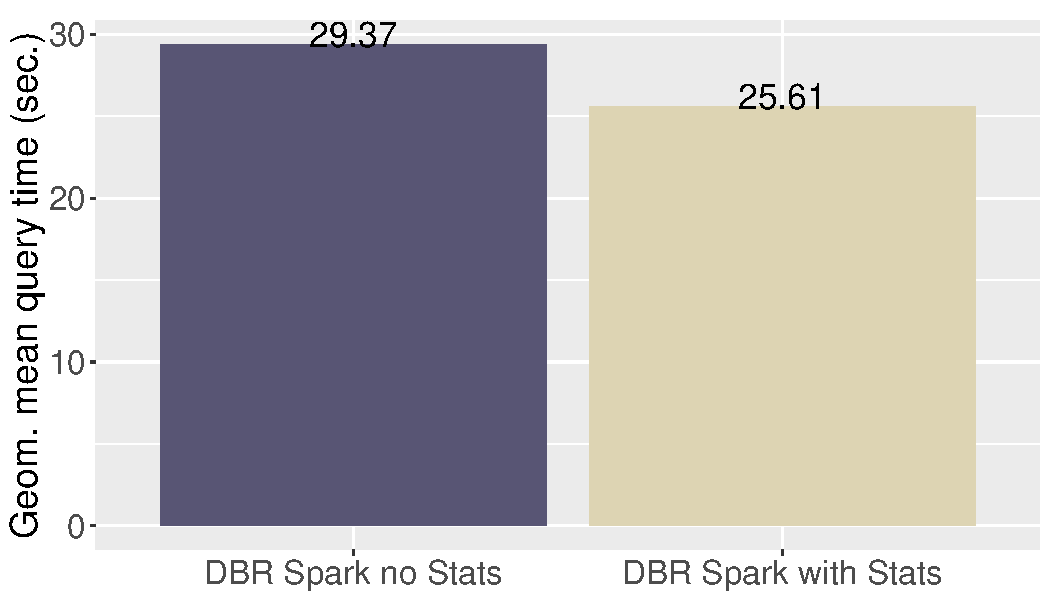
\includegraphics[width=7.0in]{imgs/additionalExperiments/statsResultsGraphs/power_geomeanTimeBarChart.pdf}}
   \end{center}
   \caption{Databricks Power Test query execution time geometric mean with and without basic statistics.}
   \label{fig:additionalResultsDatabricksWithBasicStatsPowerTestGeomean}
\end{figure}

\begin{figure}
   \begin{center}
   \scalebox{0.65}{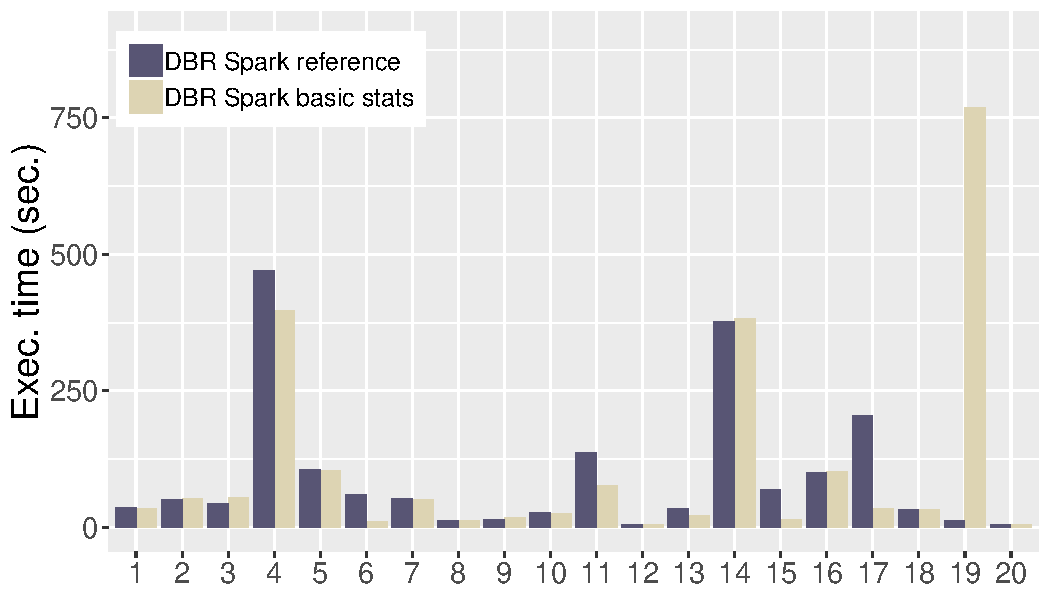
\includegraphics[width=7.0in]{imgs/additionalExperiments/basicstatsResultsGraphs/1_PDFsam_PowerTestCompAll.pdf}}
   \end{center}
   \caption{Databricks Power Test indivicual query execution times with and without basic statistics (1).}
   \label{fig:additionalResultsDatabricksWithBasicStatsPowerTestIndividualQueries1}
\end{figure}

\begin{figure}
   \begin{center}
   \scalebox{0.65}{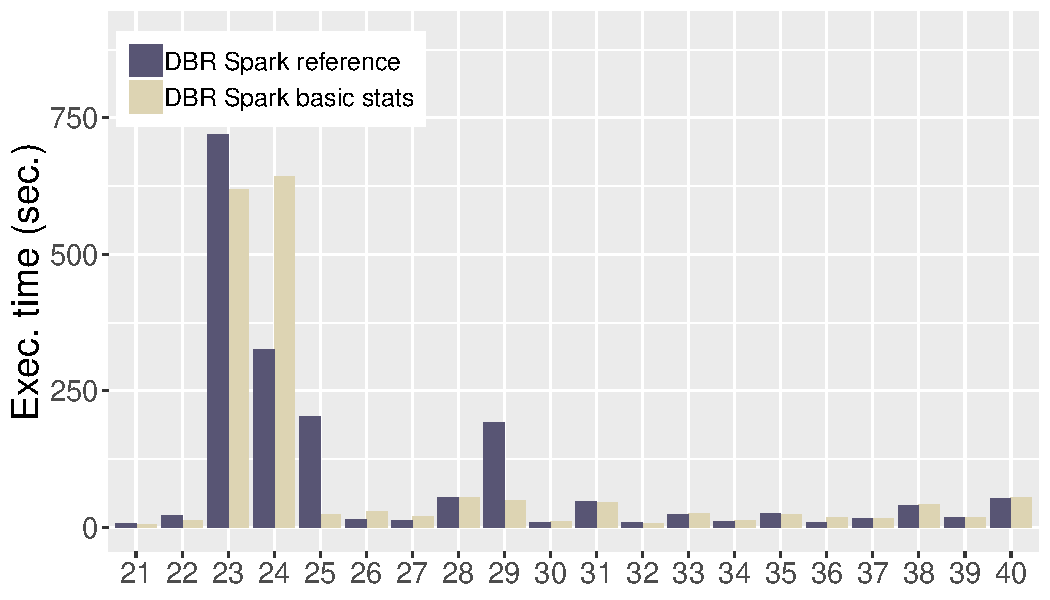
\includegraphics[width=7.0in]{imgs/additionalExperiments/basicstatsResultsGraphs/2_PDFsam_PowerTestCompAll.pdf}}
   \end{center}
   \caption{Databricks Power Test indivicual query execution times with and without basic statistics (2).}
   \label{fig:additionalResultsDatabricksWithBasicStatsPowerTestIndividualQueries2}
\end{figure}

\begin{figure}
   \begin{center}
   \scalebox{0.65}{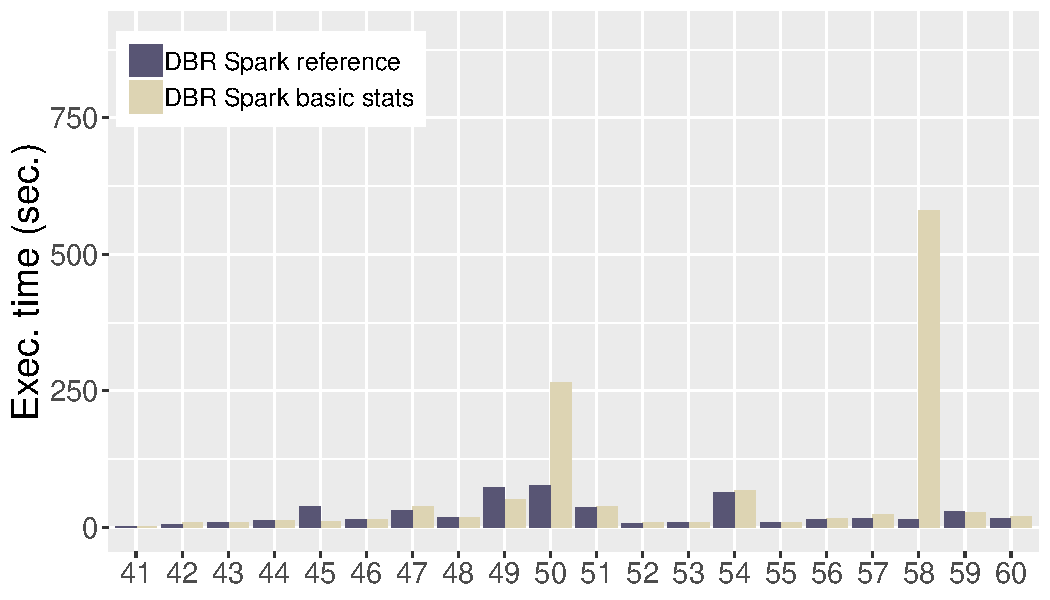
\includegraphics[width=7.0in]{imgs/additionalExperiments/basicstatsResultsGraphs/3_PDFsam_PowerTestCompAll.pdf}}
   \end{center}
   \caption{Databricks Power Test indivicual query execution times with and without basic statistics (3).}
   \label{fig:additionalResultsDatabricksWithBasicStatsPowerTestIndividualQueries3}
\end{figure}

\begin{figure}
   \begin{center}
   \scalebox{0.65}{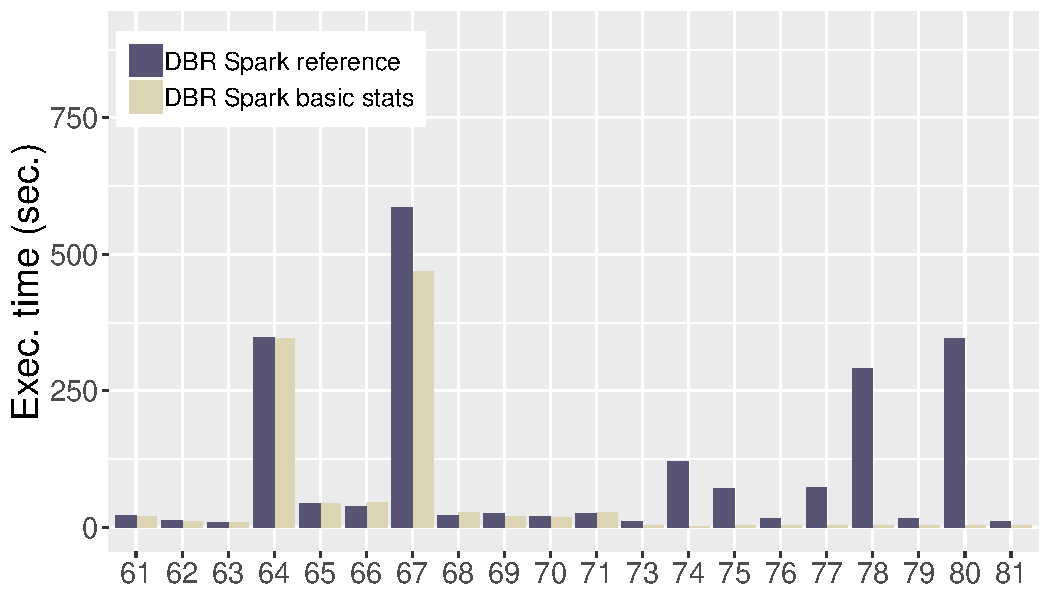
\includegraphics[width=7.0in]{imgs/additionalExperiments/basicstatsResultsGraphs/4_PDFsam_PowerTestCompAll.pdf}}
   \end{center}
   \caption{Databricks Power Test indivicual query execution times with and without basic statistics (4).}
   \label{fig:additionalResultsDatabricksWithBasicStatsPowerTestIndividualQueries4}
\end{figure}

\begin{figure}
   \begin{center}
   \scalebox{0.65}{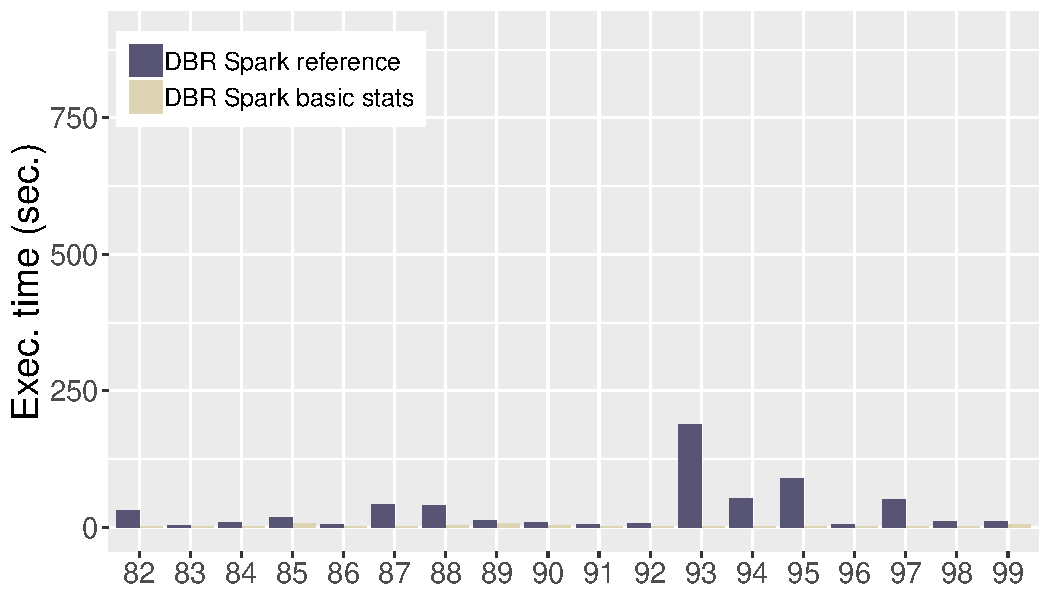
\includegraphics[width=7.0in]{imgs/additionalExperiments/basicstatsResultsGraphs/5_PDFsam_PowerTestCompAll.pdf}}
   \end{center}
   \caption{Databricks Power Test indivicual query execution times with and without basic statistics (5).}
   \label{fig:additionalResultsDatabricksWithBasicStatsPowerTestIndividualQueries5}
\end{figure}

We find severely worse performance for queries 19, 24, 50, and 58. On the other hand, queries 74 to 99 show dramatic better performance. Consequently, although basic table-level statistics do bring advantages in performance, there is a risk that they may backfire due to their limited ability to characterize a dataset. Since the generation of column-level statistics is not expensive, even when computed for all columns of all tables as we did for the TPC-DS dataset, we recommend their use.

\subsection{Databricks with cache disabled}

Databricks has an io caching feature that keeps local copies of remote files to speed up their subsequent access. The cache uses a custom format and operates automatically. The choice of i3 EC2 instances optimized for storage and equipped with NVMe SSDs responds to facilitating the use of this caching capability. It is important to point out, however, that the io cache works only with Parquet files. Thus, ORC files, which we have found to be the best choice for EMR Presto, or CSV files cannot benefit from this feature.

The io cache is enabled by default and configured to use up to half of the space available in the SSDs of the worker nodes. Since the i3.2xlarge instances we use have a 1,900 GB NVMe SSD, the available cache space is more than enough to hold the entire database, even more so in compressed form.

In our experiments for this section, we disable the io cache to analyze its effects on query processing performance. The io cache can be disabled by setting the spark.databricks.io.cache.enabled configuration property to false at the creation of the cluster. We show the effects of disabling the cache on the Power Test on Figure \ref{fig:additionalResultsDatabricksNoCachePowerTestTotalTime} to Figure \ref{fig:additionalResultsDatabricksNoCachePowerTestArithmeticMean}.

\begin{figure}
   \begin{center}
   \scalebox{0.65}{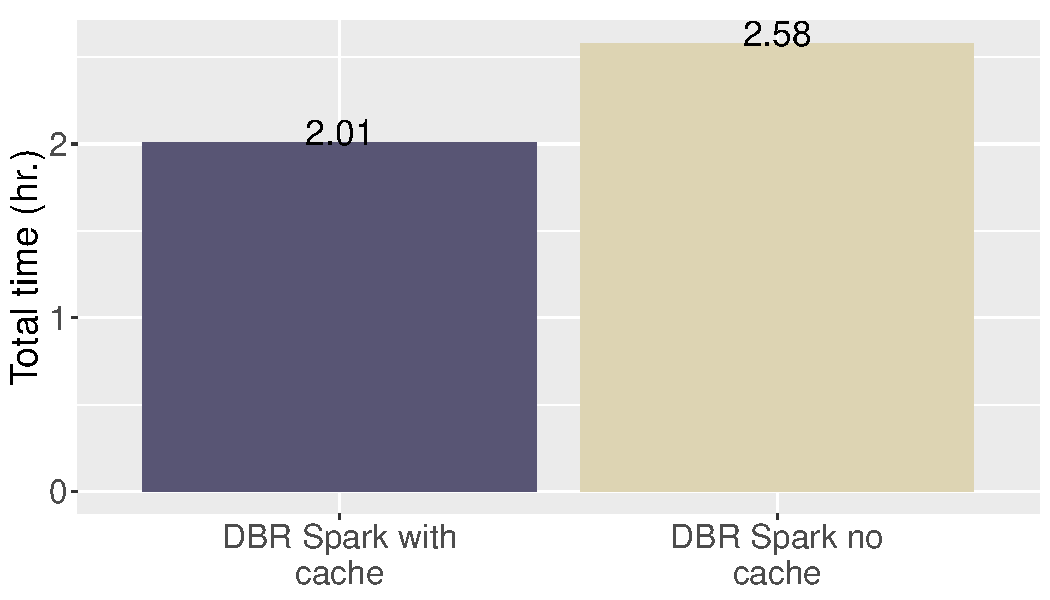
\includegraphics[width=7.0in]{imgs/additionalExperiments/nocacheResultsGraphs/power_totalHrTimeBarChart.pdf}}
   \end{center}
   \caption{Databricks Power Test total time with and without cache.}
   \label{fig:additionalResultsDatabricksNoCachePowerTestTotalTime}
\end{figure}

\begin{figure}
   \begin{center}
   \scalebox{0.65}{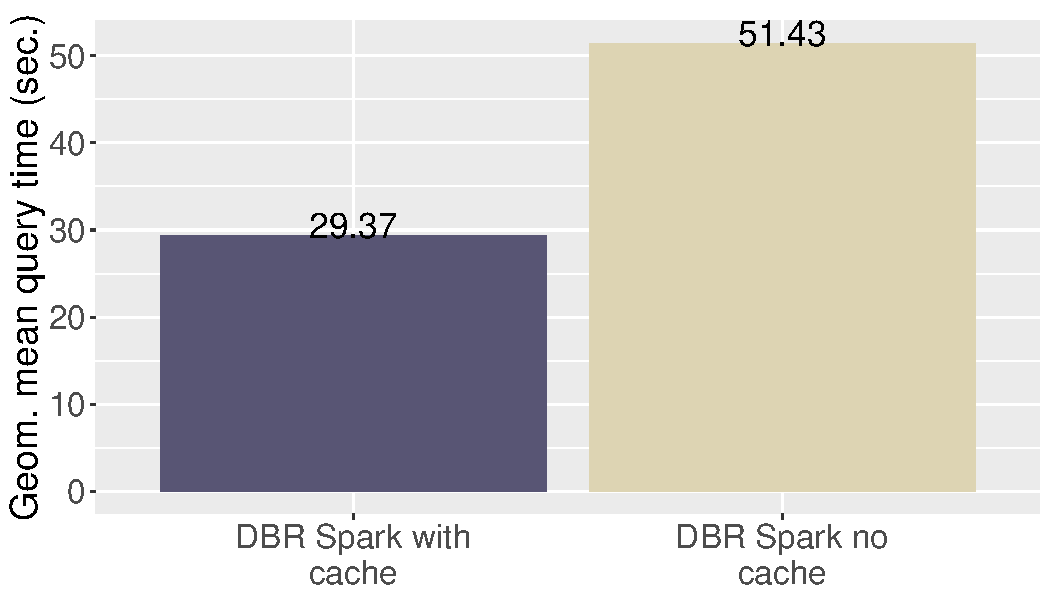
\includegraphics[width=7.0in]{imgs/additionalExperiments/nocacheResultsGraphs/power_geomeanTimeBarChart.pdf}}
   \end{center}
   \caption{Databricks Power Test query execution time geometric mean with and without cache.}
   \label{fig:additionalResultsDatabricksNoCachePowerTestGeomean}
\end{figure}

\begin{figure}
   \begin{center}
   \scalebox{0.65}{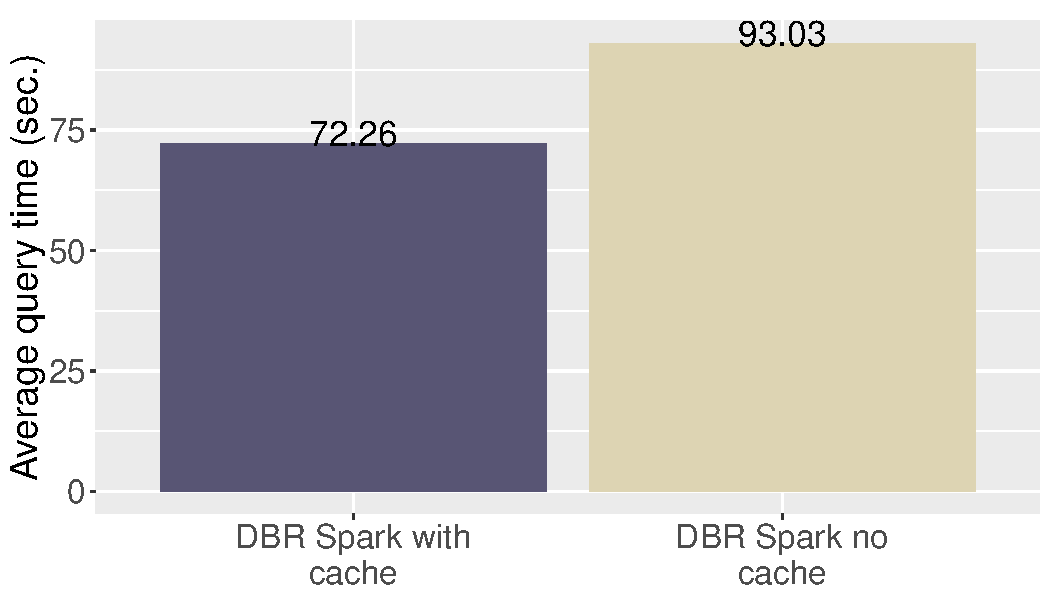
\includegraphics[width=7.0in]{imgs/additionalExperiments/nocacheResultsGraphs/power_avgTimeBarChart.pdf}}
   \end{center}
   \caption{Databricks Power Test query execution time geometric mean with and without cache.}
   \label{fig:additionalResultsDatabricksNoCachePowerTestArithmeticMean}
\end{figure}

Disabling the io cache results in a 28\% percent decline in performance, so the total time for the Power Test increases from 2 hours to about 2 and a half hours. We present the comparison for individual queries in Figure \ref{fig:additionalResultsDatabricksNoCachePowerTestIndividualQueries1} to Figure 66.

\begin{figure}
   \begin{center}
   \scalebox{0.65}{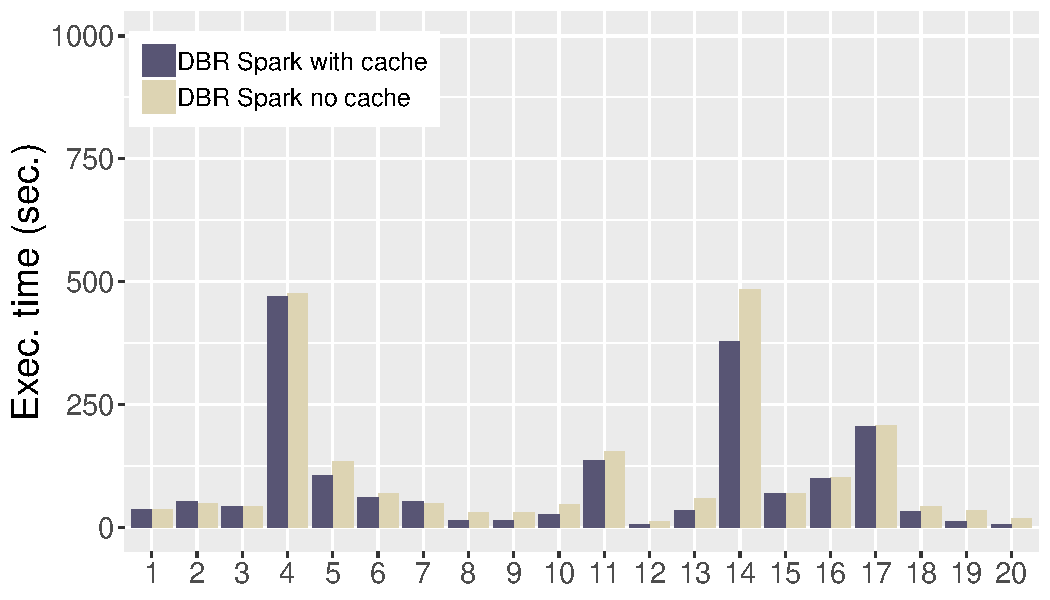
\includegraphics[width=7.0in]{imgs/additionalExperiments/nocacheResultsGraphs/1_PDFsam_PowerTestCompAll.pdf}}
   \end{center}
   \caption{Databricks Power Test individual query times with and without cache (1).}
   \label{fig:additionalResultsDatabricksNoCachePowerTestIndividualQueries1}
\end{figure}

\begin{figure}
   \begin{center}
   \scalebox{0.65}{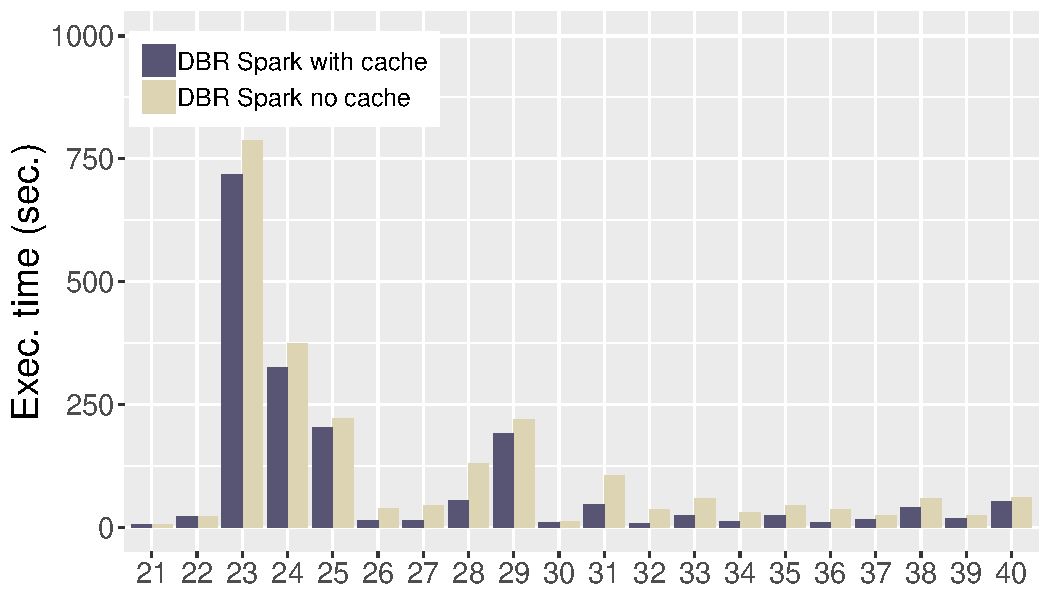
\includegraphics[width=7.0in]{imgs/additionalExperiments/nocacheResultsGraphs/2_PDFsam_PowerTestCompAll.pdf}}
   \end{center}
   \caption{Databricks Power Test individual query times with and without cache (2).}
   \label{fig:additionalResultsDatabricksNoCachePowerTestIndividualQueries2}
\end{figure}

\begin{figure}
   \begin{center}
   \scalebox{0.65}{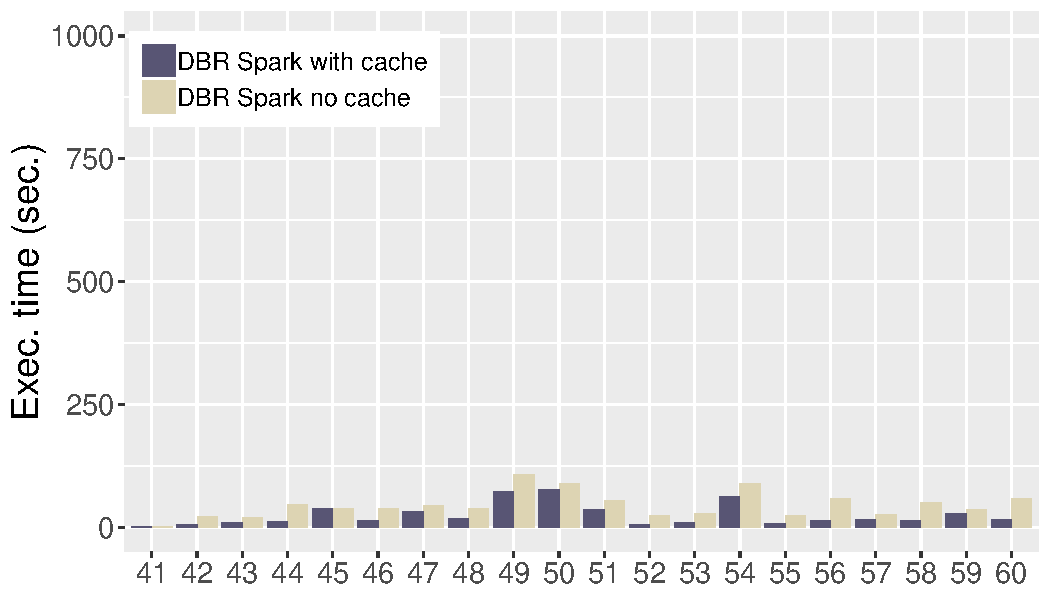
\includegraphics[width=7.0in]{imgs/additionalExperiments/nocacheResultsGraphs/3_PDFsam_PowerTestCompAll.pdf}}
   \end{center}
   \caption{Databricks Power Test individual query times with and without cache (3).}
   \label{fig:additionalResultsDatabricksNoCachePowerTestIndividualQueries3}
\end{figure}

\begin{figure}
   \begin{center}
   \scalebox{0.65}{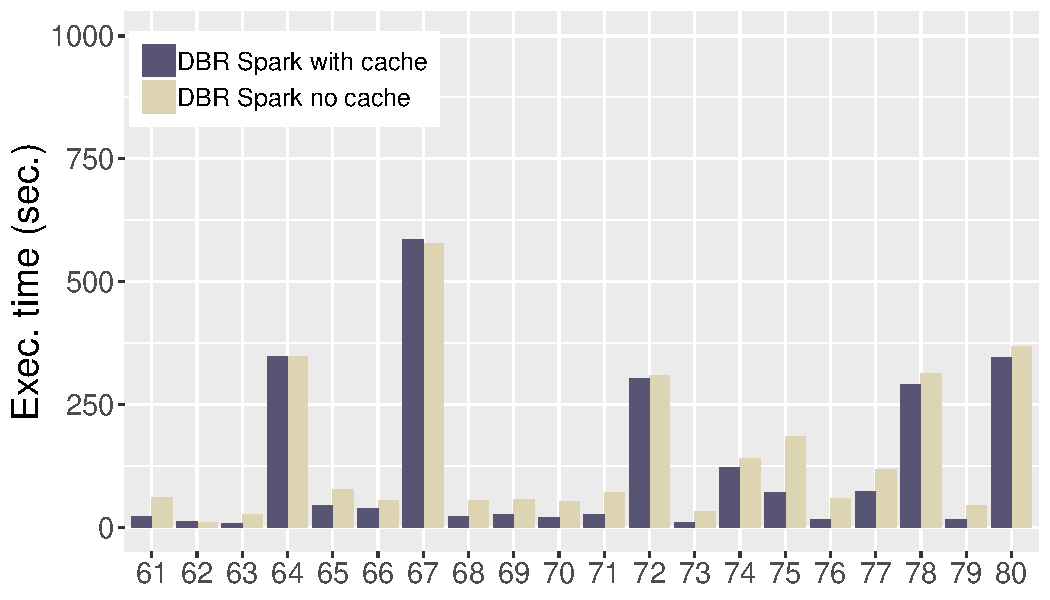
\includegraphics[width=7.0in]{imgs/additionalExperiments/nocacheResultsGraphs/4_PDFsam_PowerTestCompAll.pdf}}
   \end{center}
   \caption{Databricks Power Test individual query times with and without cache (4).}
   \label{fig:additionalResultsDatabricksNoCachePowerTestIndividualQueries4}
\end{figure}

\begin{figure}
   \begin{center}
   \scalebox{0.65}{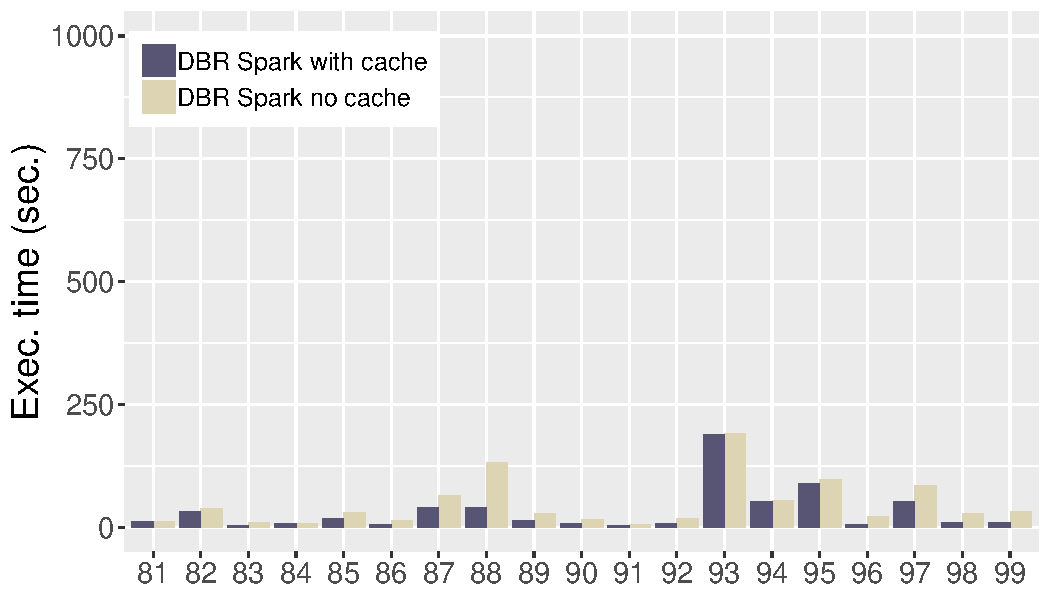
\includegraphics[width=7.0in]{imgs/additionalExperiments/nocacheResultsGraphs/5_PDFsam_PowerTestCompAll.pdf}}
   \end{center}
   \caption{Databricks Power Test individual query times with and without cache (5).}
   \label{fig:additionalResultsDatabricksNoCachePowerTestIndividualQueries5}
\end{figure}

A total of 53 queries show a decrease in performance of at least 50\% when the cache is disabled, 42 of them take twice as long to complete. Queries 32, 42, and 56 take more than 4 times as long. Only in two cases we saw a drop in performance larger than 10\% when using the cache, namely for queries 21 and 62. Cache misses or overhead in caching files for successive queries could explain that. Overall, the results show that the io cache offers a significant improvement for Databricks. When comparing with EMR Presto in our reference results, it is clear that although it represents an advantage, it is by no means the deciding factor. The Power Test takes almost 3 times as much time in EMR Presto as in Databricks without io cache.

In the Throughput Test we also witness significant performance degradation when the io cache is disabled, as depicted in Figure \ref{fig:additionalResultsDatabricksNoCacheTputTest}. Predictably, the performance degradation is larger in the Throughput Test when compared with the Power Test, 35\% vs. 28\%, due to multiple instances of the same queries being able to take advantage of the cache.

\begin{figure}
   \begin{center}
   \scalebox{0.65}{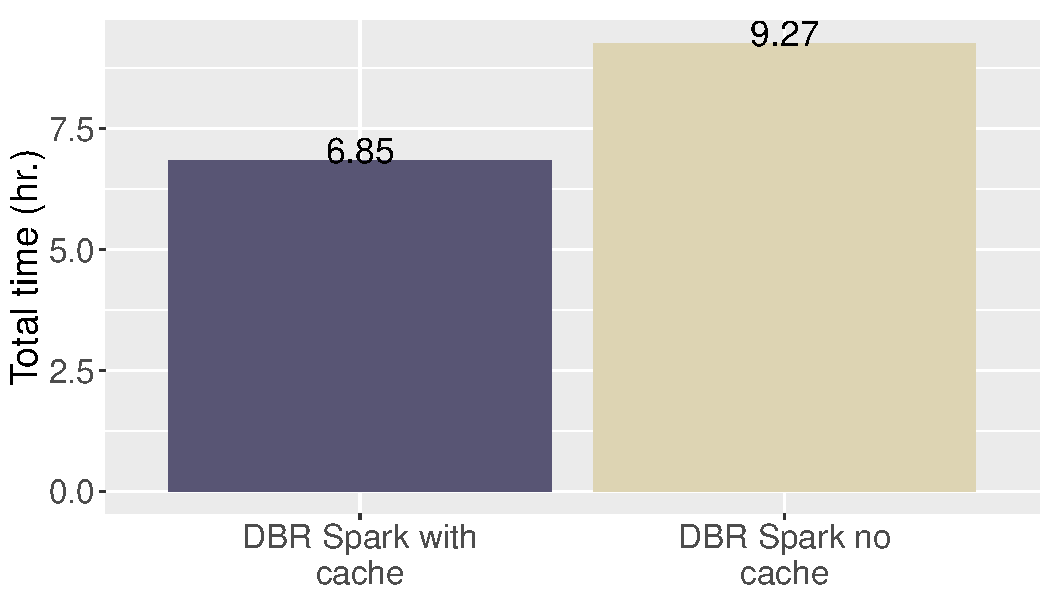
\includegraphics[width=7.0in]{imgs/additionalExperiments/nocacheResultsGraphs/tput_totalHrTimeBarChart.pdf}}
   \end{center}
   \caption{Databricks Throughput Test total time with and without cache.}
   \label{fig:additionalResultsDatabricksNoCacheTputTest}
\end{figure}

\subsection{Parquet vs. ORC format in EMR Presto}

Our reference results use the ORC format for EMR Presto, which we found to be a better alternative than Parquet from a performance standpoint. Nevertheless, it is interesting to analyze the behavior of EMR Presto with the Parquet format to determine the effect a different column-based storage format can have.

\begin{figure}
   \begin{center}
   \scalebox{0.65}{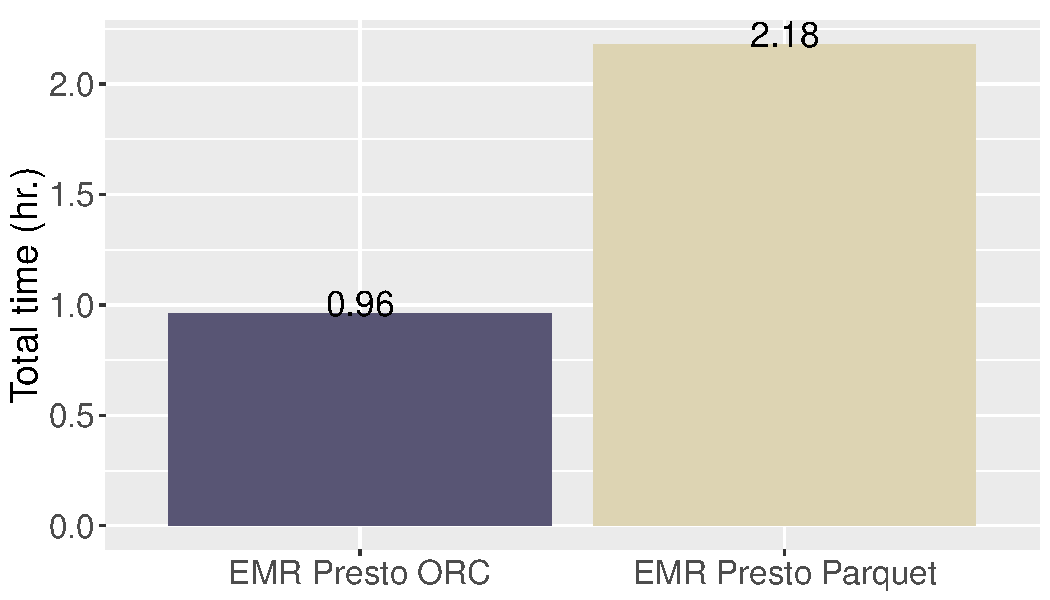
\includegraphics[width=7.0in]{imgs/additionalExperiments/orcvsparquetResultsGraphs/load_totalHrTimeBarChart.pdf}}
   \end{center}
   \caption{EMR Presto Data Loading Test total time with ORC vs. Parquet.}
   \label{fig:additionalResultsPrestoORCvsParquetDataLoading}
\end{figure}

Figure \ref{fig:additionalResultsPrestoORCvsParquetDataLoading} provides the data loading times for EMR Presto using ORC and alternatively using Parquet, again using the 1 TB dataset. The use of Parquet more than doubles the required time when compared to using the ORC format (our reference result). This is likely due to a more mature and optimized implementation for ORC in Presto, since as we saw on Section \ref{referenceResultsDataLoading}, even better results can be achieved for Parquet using Databricks. Hence, it is not due to the drawbacks of the format itself.

The total execution time for the Power Test using both formats is shown in Figure \ref{fig:additionalResultsPrestoORCvsParquetPowerTestTotalTime}, followed by the geometric mean and the arithmetic mean of query completion times in Figure \ref{fig:additionalResultsPrestoORCvsParquetPowerTestGeomean} and Figure \ref{fig:additionalResultsPrestoORCvsParquetPowerTestArithmeticMean}, respectively.

\begin{figure}
   \begin{center}
   \scalebox{0.65}{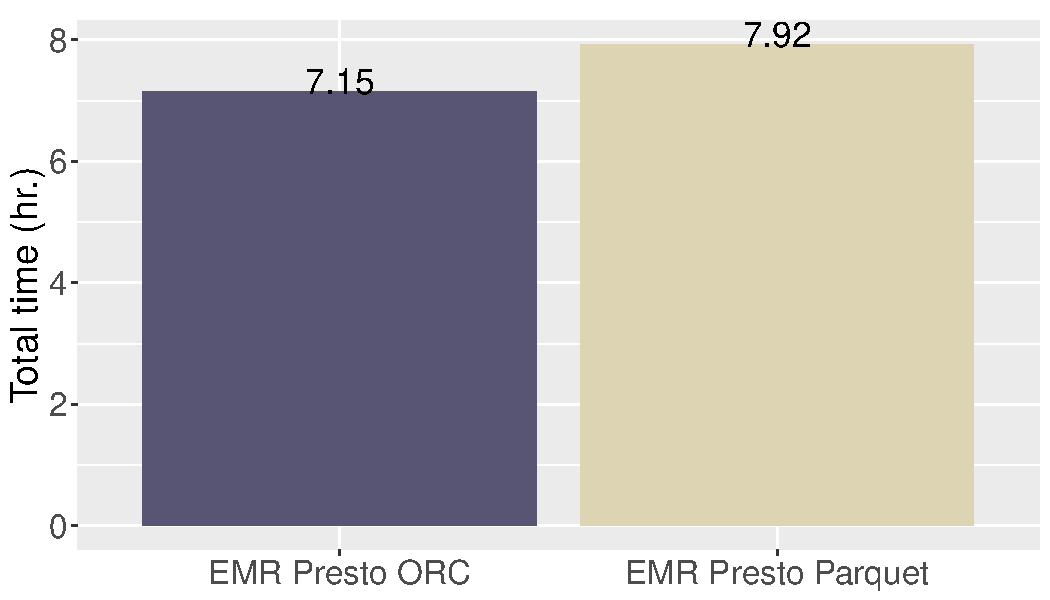
\includegraphics[width=7.0in]{imgs/additionalExperiments/orcvsparquetResultsGraphs/power_totalHrTimeBarChart.pdf}}
   \end{center}
   \caption{EMR Presto Power Test total time with ORC vs. Parquet}
   \label{fig:additionalResultsPrestoORCvsParquetPowerTestTotalTime}
\end{figure}

\begin{figure}
   \begin{center}
   \scalebox{0.65}{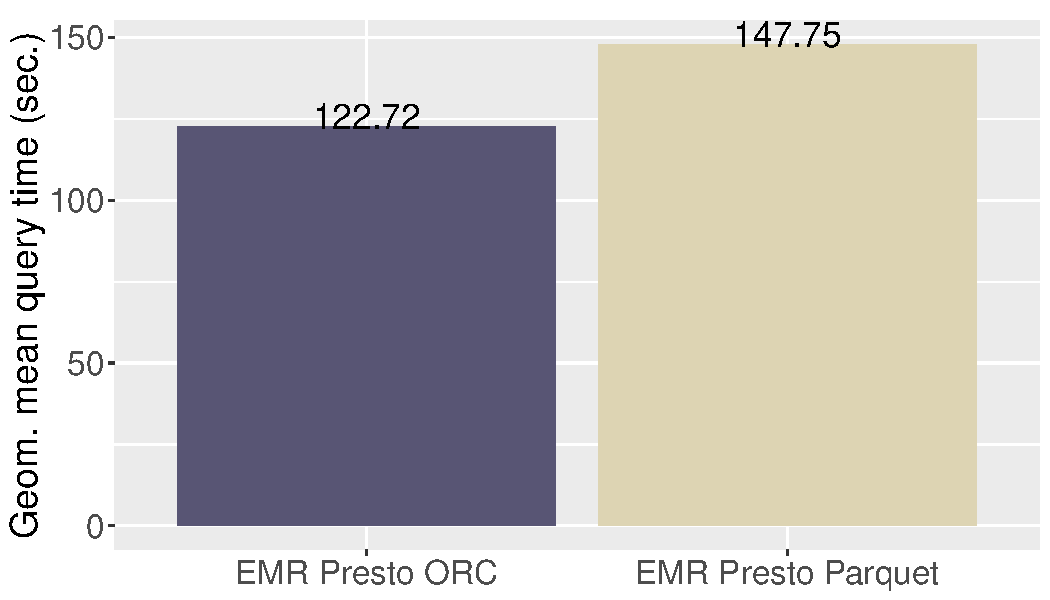
\includegraphics[width=7.0in]{imgs/additionalExperiments/orcvsparquetResultsGraphs/power_geomeanTimeBarChart.pdf}}
   \end{center}
   \caption{EMR Presto Power Test query execution time geometric mean with ORC vs. Parquet.}
   \label{fig:additionalResultsPrestoORCvsParquetPowerTestGeomean}
\end{figure}

\begin{figure}
   \begin{center}
   \scalebox{0.65}{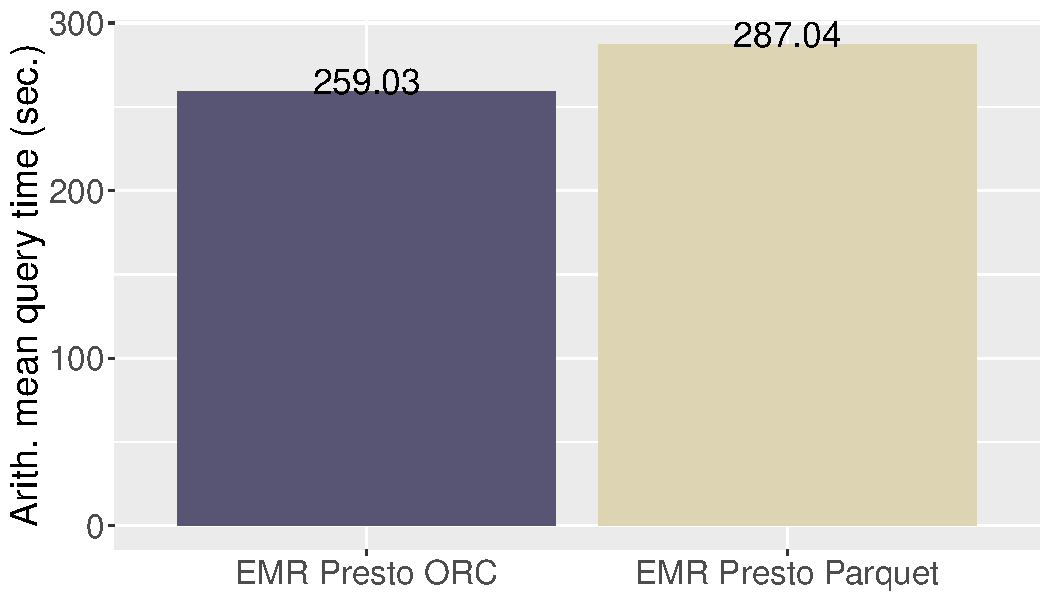
\includegraphics[width=7.0in]{imgs/additionalExperiments/orcvsparquetResultsGraphs/power_avgTimeBarChart.pdf}}
   \end{center}
   \caption{EMR Presto Power Test query execution time arithmetic mean with ORC vs. Parquet.}
   \label{fig:additionalResultsPrestoORCvsParquetPowerTestArithmeticMean}
\end{figure}

We observe a relatively small decrease in performance with the use of the Parquet format of about 10\%. We omit the detailed comparison for each query since for the most part we observe a regular behavior repeated across all queries. Only 10 queries showed a better performance with Parquet, with only query 51 showing an improvement beyond 10\%, 19\% to be exact.

In regards to the Throughput Test, we present the results in Figure \ref{fig:additionalResultsPrestoORCvsParquetTputTest}. We can see that with 4 concurrent streams running, the degradation of performance when using Parquet increases to about 13\%.

\begin{figure}
   \begin{center}
   \scalebox{0.65}{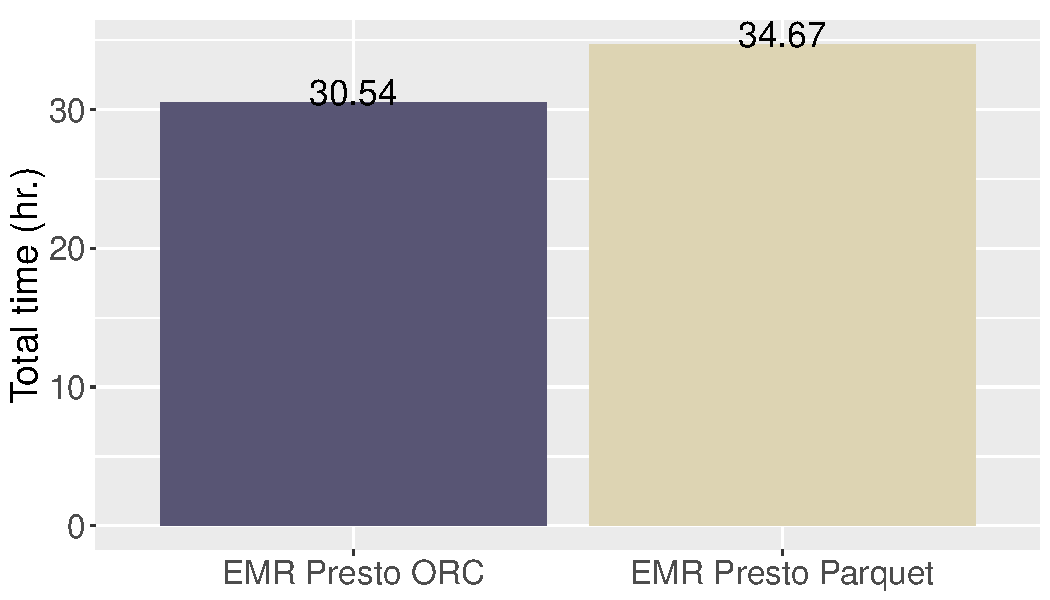
\includegraphics[width=7.0in]{imgs/additionalExperiments/orcvsparquetResultsGraphs/tput_totalHrTimeBarChart.pdf}}
   \end{center}
   \caption{EMR Presto Throughput Test total time with ORC vs. Parquet}
   \label{fig:additionalResultsPrestoORCvsParquetTputTest}
\end{figure}

From the previous results, we can conclude that ORC is a better option for EMR Presto than Parquet, with a major improvement in loading times and a small but valuable improvement for query processing. In cases when a database already exists in the Parquet format, converting to ORC is probably not worth it. The large differences in performance between EMR Presto and Databricks are also not the result of using different column-storage data formats.

\subsection{S3 vs. HDFS storage in EMR Presto}

